\documentclass[a4paper,11pt]{article}
\usepackage{amssymb}
\usepackage{latexsym}
\usepackage{eufrak}
\usepackage{euscript}
\usepackage{exscale}
\usepackage{graphicx}
\usepackage{mathrsfs}
\usepackage{epsfig}
\usepackage{hyperref}
\usepackage{adjustbox}

\usepackage[hypcap]{caption}
\usepackage{fancyhdr}
\usepackage[german]{babel}
\usepackage[latin1,utf8]{inputenc}
\usepackage{pdfpages}
\usepackage{amsthm}
\usepackage{color}
\usepackage{listings}
\usepackage{float}
\usepackage{titlesec}
\usepackage{apacite}


\lstset{
basicstyle=\scriptsize\tt,
}

\lstset{ %
  language=R,                     % the language of the code
  basicstyle=\footnotesize,       % the size of the fonts that are used for the code
  numbers=left,                   % where to put the line-numbers
  numberstyle=\tiny\color{gray},  % the style that is used for the line-numbers
  stepnumber=1,                   % the step between two line-numbers. If it's 1, each line
                                  % will be numbered
  %firstnumber=\numexpr\inputlineno+1\relax
  numbersep=5pt,                  % how far the line-numbers are from the code
  %backgroundcolor=\color{white},  % choose the background color. You must add \usepackage{color}
  showspaces=false,               % show spaces adding particular underscores
  showstringspaces=false,         % underline spaces within strings
  showtabs=false,                 % show tabs within strings adding particular underscores
  %frame=single,                   % adds a frame around the code
  rulecolor=\color{black},        % if not set, the frame-color may be changed on line-breaks within not-black text (e.g. commens (green here))
  tabsize=1,                      % sets default tabsize to 2 spaces
  captionpos=NA,                   % sets the caption-position to bottom
  breaklines=true,                % sets automatic line breaking
  breakatwhitespace=false,        % sets if automatic breaks should only happen at whitespace
  title=\lstname,                 % show the filename of files included with \lstinputlisting;
                                  % also try caption instead of title
  keywordstyle=\color{blue},      % keyword style
%  commentstyle=\color{dkgreen},   % comment style
  %stringstyle=\color{red},      % string literal style
  escapeinside={\%*}{*)},         % if you want to add a comment within your code
  morekeywords={*,...}            % if you want to add more keywords to the set
} 


\pagestyle{fancy}
%\pagenumbering{arabic}
%\rhead{\small{\today}}
\chead{}
\lhead{\small{Statistics, Visualization and more using R}}
\rhead{Bradley Mackay, Clemens Ehlich}
\rfoot{\small{\textcolor{gray}{clemens.ehlich@sbg.ac.at \\ bradley.mackay@sbg.ac.at}}}
\lfoot{\small{\textcolor{gray}{Master Data Science \\ PhD Linguistics \\ Universität Salzburg 
}}}
\renewcommand{\headrulewidth}{0.4pt}
\renewcommand{\footrulewidth}{1pt}
\setlength{\headwidth}{420pt}
%\newcommand{\sectionbreak}{\clearpage}

\markright{}


\setlength{\textheight}{665pt}
\setlength{\textwidth}{440pt}
\setlength{\marginparwidth} {10pt}
\setlength{\hoffset}{-30pt}
\setlength{\voffset}{-50pt}
\fancyhfoffset[R]{0.5mm} 
\setlength{\headsep}{1cm}

\newtheorem{defin}{Definition}[section]
\newtheorem{satz}[defin]{Theorem}
\newtheorem{folg}[defin]{Proposition}
\newtheorem{bem}[defin]{Bemerkung}
\newtheorem{lem}[defin]{Lemma}
\newtheorem{hs}[defin]{Lemma}
\newtheorem*{remark}{Bemerkung}



\hyphenation{bio-mim-ic-ry bio-in-spi-ra-tion re-us-a-ble pro-vid-er ha-ving con-si-de-ring
 cor-res-pon-ding}

\begin{document}
\hrule
\begin{center}
\Large{\textbf{Statistics, Visualization and more using R}} \\[3mm]
\hrule
\hrule 
\vspace{2mm}
\LARGE{\textbf{R Packages: A Beginner's Guide }} \\[2mm] 
\hrule
\hrule
\vspace{6mm}
\large{ \textbf{Bradley Mackay, Clemens Ehlich}	
}\\[5mm]

\end{center}
\begin{center}
\today
\end{center}
\hrule
\vspace{3cm}


\begin{center}
\large{\textbf{Summary}}
\end{center}
One of the biggest advantages of the R programming language is the extensive number of extension packages available which make tasks in R  much easier. R packages are collections of functions and datasets and are mostly created by the community itself. As the title suggests, this short paper is about how to create your own little R package, because creating your own package has many advantages. Especially if you have to work on recurring tasks. For this we will first give a summary of important commands to work with packages. Then we will give an overview how packages are built and finally we will give a step by step guide how to create your first own package.
\\
\\
\\
%\begin{center}
%	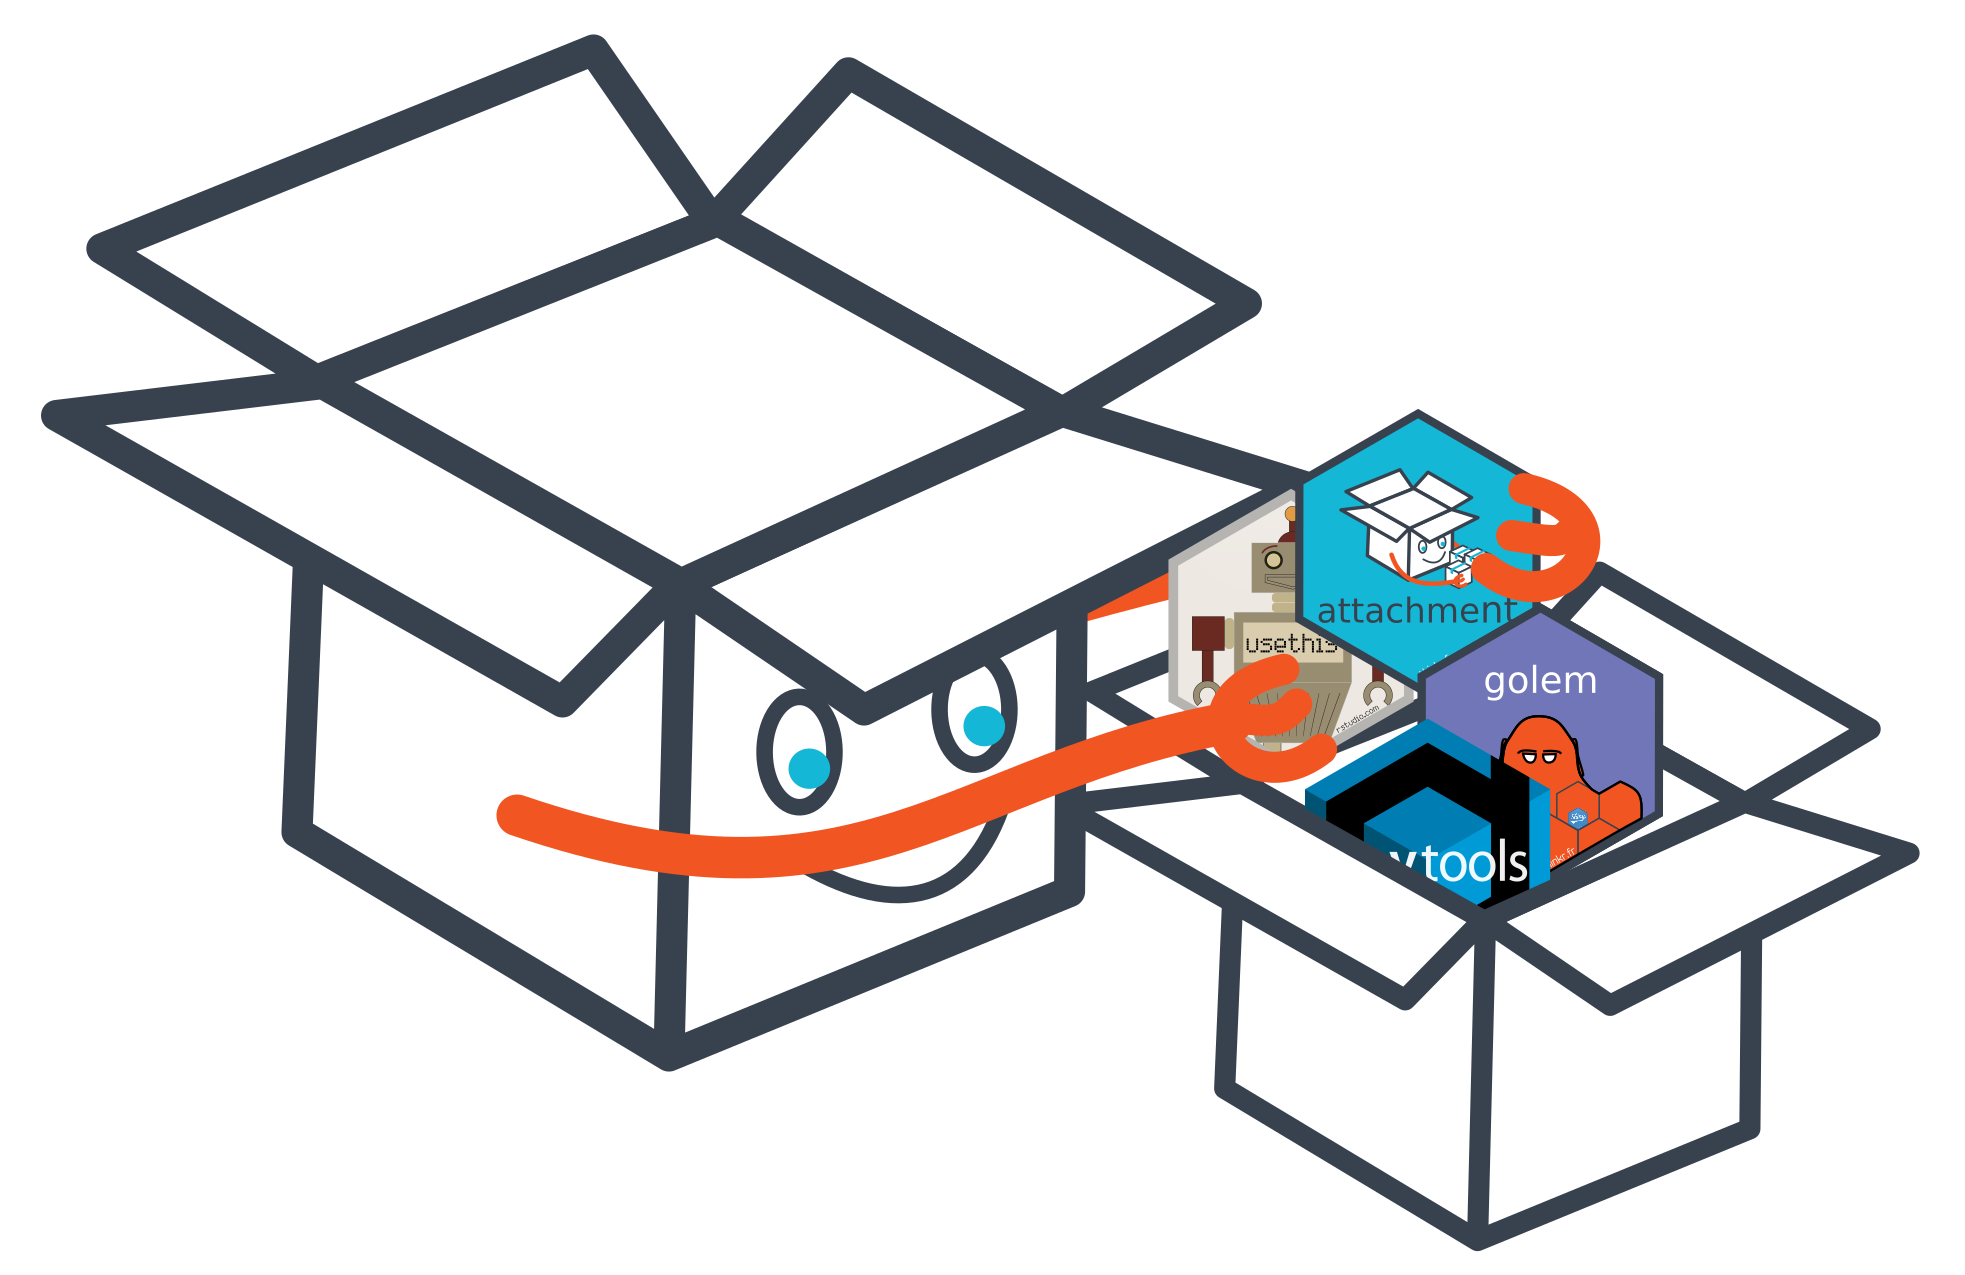
\includegraphics[width=0.6\linewidth]{pack}
%\end{center}  
\pagebreak
\tableofcontents
\vspace*{2cm}
%\clearpage
\nopagebreak
\section{Basics}
\subsection{What's a package}

R packages are collections of functions and data sets. They extend the basic functionalities of the Language itself or add new ones. Packages are usually written in R code, but there are packages which extend this functionality to other languages for example, C++ (with the \texttt{rcpp} package \cite{Rcpp} ). As a general rule of thumb, if there are any functions which you have copied and pasted from other R scripts more than twice, you should consider creating a package for those functions.

\subsection{Why Packages?}
Using packages makes your work-flow a lot easier and faster. Because for  recurring tasks its not necessary to reinvent the wheel again and again. There are more than 19.000 packages on CRAN. For nearly every common problem a package exist, for example to load or visualize data. Packages form also interfaces to other software and their file formats (foreign, caffe, RQGIS), databases (RODBC, RPostgreSQL, etc), other programming languages (Rcpp, RPython) or webservices (Rfacebook, RGoogleAnalytics).

\subsection{Where can I find packages?}

To get an overview of which packages are already available you can use the website \textit{https://www.rdocumentation.org/}. It lists nearly every package exists. You can also look at \textit{https://cran.r-project.org} the official R Website or  
BioConductor a website for Biology Content (\textit{http://bioconductor.org/}). Of course there are also countless packages on GitHub (\textit{https://github.com/}).

\subsection{Some important R-Commands to work with packages}


%\begin{lstlisting}[frame=single]
%# Installing Packages:
%install.packages("xyz") 
%install.packages(c("xyz", "123"))
%
%# check and update Packages:
%old.packages("xyz")
%update.packages("xyz")
%
%# remove Packages:
%remove.packages("xyz")
%\end{lstlisting}
There is one big problem: each repository (CRAN, BioConductor, etc) has its own way to install a package from them. To simplify this process you can use the package $ "devtools" $. But for this you might also need to install $ "Rtools" $ for Windows, $ "Xcode" $ for Mac or if you using Linux $"r-devel"$ for Linux. But then you can install packages directly from the repository with the following code: 


\begin{lstlisting}[frame=single]
install_bioc() #from Bioconductor
install_cran() #from CRAN
install_github() #from GitHub
install_local() #from a local file
install_url() #from a URL
\end{lstlisting}

\section{Making you own Package}
\subsection{What does a package consist of?}
In this chapter we want to show how to create your own package. For this it is important to know how a package is built. If you create a new file to create an R-package, a folder structure is automatically created in the background. This folder structure is shown in figure \ref{structure}. The DESCRIPTION-File, the NAMESPACE, the FUNCTIONS and the MANUALS are mandatory. The rest, which are dotted in the graphic, is optional.
\\
\begin{figure}
\begin{center}
	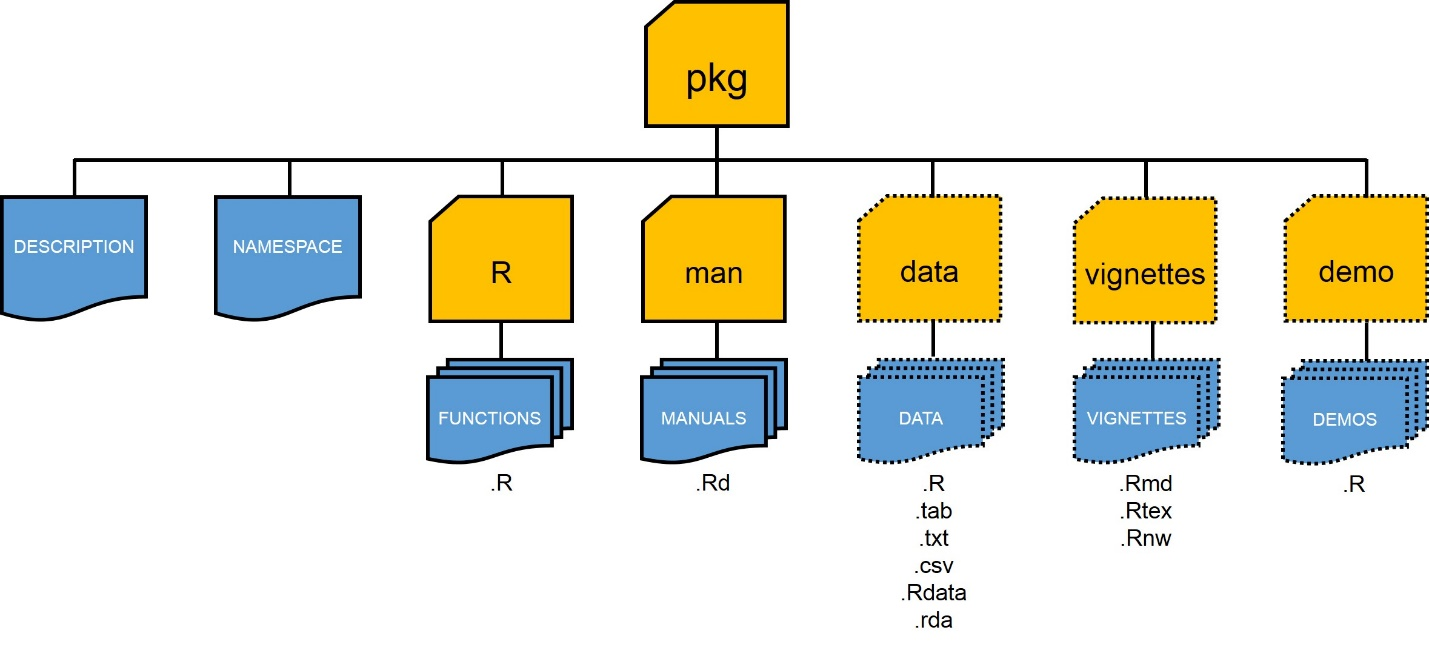
\includegraphics[width=.7\linewidth]{stott}
	\caption{Package file structure}
	\label{structure}
\end{center}  
\end{figure}

While it is possible to write a package from scratch, there are a number of packages available which make the process much easier. By making use of functionality in \texttt{devtools} \cite{devtools}, \texttt{usethis} \cite{usethis} and \texttt{roxygen2} \cite{roxygen2}, almost all of the manual input is kept to a bare minimum. It is perfectly possible to have a functioning package (with no frills!) up and running in about 10 mins using the functions provided by these three packages. In terms of beginning a package project, there are several different ways to initialise a \texttt{.Rproj} which will require slightly altered ways which you need to use \texttt{roxygen2} in the initial project set up. For clarity, the work-flow described here is for those initialising a new .Rproj as an R package in a clear directory.

\subsection{Initial setting up}
Initialising a new R package project will give you the bare-bones file structure required to make a package, as illustrated in \ref{structure}. The file structure was however not created with \texttt{roxygen2} and so there is some initial set up required to get round this. Firstly, buildtools needs to be configured to use \texttt{roxygen2} functionality, it's a good idea to also initialise a github repository for your package at this point if that is part of your intended work-flow. A feature of \texttt{roxygen2} is that it will not overwrite any files that it did not create, while this is beneficial if you are switching to \texttt{roxygen2} in a package that you have been previously building without it, it means that we need to delete some of the existing shell so that \texttt{roxygen2} can create these files itself. The shell files include the NAMESPACE file as well as the .Rd file in the man folder (leaving this file would not cause any issues to your package run but it is superfluous to the package structure requirements). The existing "Hello World" .R file in the R folder (from where the .Rd file was created) can also be deleted, or just renamed and overwritten with your first function. Best practice for functions is to have one file per function, but they can happily stay in one file. All manual additions are made to files in the R folder, .Rd files in the man folder are read only and are generated by \texttt{roxygen2}. If you open one of these .Rd files you will see that the syntax is loosely based on \LaTeX  syntax. Calling \texttt{devtools::document()} (which actually itself calls \texttt{roxygen2::roxygenise()}) at this point will rewrite NAMESPACE and the basic required structure will be once more intact.

\section{Adding content \& roxygensing your functions}
Once you have a function that you want to include as part of your package, you need to tell \texttt{roxygen2} to include it. This is easily done by adding a roxygen block to your function:

\begin{lstlisting}[frame=single]
#' Title
#'
#' @param
#' @return
#' @examples
#' @export
\end{lstlisting}

This roxygen skeleton can be inserted by putting your cursor anywhere in the function and then clicking code then  $Insert Roxygen Skeleton $. running \texttt{devtools::document()} again will roxygenise your function and create a .Rd file in the man folder. The information you enter here will appear in the help files of your package. You may get a warning if you haven't started \texttt{\#' \@param} \texttt{\#' \@return} with a capital letter and ended with a full stop. A useful function which should be run often, and certainly after roxygenising functions, is \texttt{devtools::check()}, this installs and restarts your package and then performs a check on your code. It will then give you feedback on whether your package check has exited with a 0 or 1 status and give you either the error, warning or note that has been generated. You can simply work your way through each of these messages until your check passes clean.



\subsection{Further development}

Ultimately the amount of time invested in writing supplementary files that are not essential to the basic functioning of your package depends on the final destination you envisage for your package. If you plan to keep your package available only in your local files, there is little to no point in providing extensive vignettes for each function for example. Similarly, if you'd be content to live with any number of warnings when you call your package, then you may not feel it necessary to spend time cleaning up your file structure to pass \texttt{devtools::check()} without warnings. If you plan to release your package into the wild however, your package structure needs to adhere to much stricter package checks, certainly if you plan to submit to CRAN, there will be a greater number of supplementary checks and files that need to be included in your package. On this note, there seems to be very mixed reactions to CRAN's submission process. Although CRAN developers are actively encouraging submissions, a cursory search of the \#CRAN handle on twitter suggests that even very well established members of the R community, including staff on the Rstudio team, have had very negative experiences of pushing their packages to CRAN.

\subsubsection{Checking package names}
If you do plan to release your package, you need to check first of all that your planned package name is available on (ideally) all platforms. Rather than having to go to each site individually, there is a handy package named \texttt{available} \cite{available} which has a few useful functions. The most useful of these is \texttt{available::available()}. This function does two things, it first checks github, Bioconductor and CRAN and tells you if your name is available or not. It also checks a number of websites including urbandictionary.com to see if your name has any offensive meanings you may not be aware of. It also optionally opens these pages in your web browser (you can turn this option off with \texttt{browse = FALSE}). you can optionally do a target search e.g. \texttt{available::available\_on\_github()}. Once you have done these checks, your package is theoretically ready to go.

\subsection{Making your package more attractive to users}
If you want people to actually use the package you have created, rather than someone else's package which may have similar functionality, it's a good idea to make your package as accessible as possible to your intended users. This means initializing an informative README and creating vignettes to walk the reader through the main functions in your package. READMEs can easily be generated with the \texttt{usethis::use\_readme\_rmd()}. This will create both a .rmd and a .md file in the main directory. You can edit the .rmd file and it will automatically update the .md file. There is a similar function from \texttt{usethis::use\_vignette()} which automatically generates a vignette for you to complete. All this information will then be available to users once they have installed your package through the \texttt{help()} function, but to call attention to your package in the first place is also important. The \texttt{pkgdown} package \cite{pkgdown} can help tremendously here. \texttt{pkgdown} takes the README and any vignettes you have initialised along with your description file and turns them into a static HTML site. This site can then be hosted free of charge on github pages. This is simply executed by calling \texttt{pkgdown::build\_site()}. You may also want to think about creating a hex logo for your package, while it is absolutely not necessary, a good hex logo could help your package stand out in a crowded market. There is a \texttt{hexSticker} package \cite{hexSticker} which will help you here but hex stickers could be simply created as .png files in photoshop. If you have initialised a pkgdown site you may need to add some of the files it creates to build ignore (unless you don't mind getting a note/ warning!).

\subsection{Once your package is done}
Once you have a package which contains useful, well-documented functionality, and which is hosted in a way that allows people to make use of it, there are a number of options available to track and store usage metrics. If your package is available through github you can track downloads through packages such as \texttt{badger} which allow you to embed badges into your README file. Badges are also capable of tracking downloads from CRAN and Bioconductor and these metrics can be broken down by month or year. To track package usage straight from CRAN or Bioconductor, there are packages such as \texttt{cranlogs} \cite{cranlogs} and \texttt{dlstats}, which have the advantage of providing data in a format which can be stored and visualised in R or further processed into (for example) a Shiny app and tracked that way.

\bibliographystyle{apacite}
\bibliography{refs}


%\begin{thebibliography}{laengste Labelbreite}
%   \bibitem[trial]{Something about this here I don't know}
%\end{thebibliography}


\end{document}

